% Options for packages loaded elsewhere
\PassOptionsToPackage{unicode}{hyperref}
\PassOptionsToPackage{hyphens}{url}
%
\documentclass[
]{article}
\usepackage{amsmath,amssymb}
\usepackage{iftex}
\ifPDFTeX
  \usepackage[T1]{fontenc}
  \usepackage[utf8]{inputenc}
  \usepackage{textcomp} % provide euro and other symbols
\else % if luatex or xetex
  \usepackage{unicode-math} % this also loads fontspec
  \defaultfontfeatures{Scale=MatchLowercase}
  \defaultfontfeatures[\rmfamily]{Ligatures=TeX,Scale=1}
\fi
\usepackage{lmodern}
\ifPDFTeX\else
  % xetex/luatex font selection
\fi
% Use upquote if available, for straight quotes in verbatim environments
\IfFileExists{upquote.sty}{\usepackage{upquote}}{}
\IfFileExists{microtype.sty}{% use microtype if available
  \usepackage[]{microtype}
  \UseMicrotypeSet[protrusion]{basicmath} % disable protrusion for tt fonts
}{}
\makeatletter
\@ifundefined{KOMAClassName}{% if non-KOMA class
  \IfFileExists{parskip.sty}{%
    \usepackage{parskip}
  }{% else
    \setlength{\parindent}{0pt}
    \setlength{\parskip}{6pt plus 2pt minus 1pt}}
}{% if KOMA class
  \KOMAoptions{parskip=half}}
\makeatother
\usepackage{xcolor}
\usepackage[margin=1in]{geometry}
\usepackage{longtable,booktabs,array}
\usepackage{calc} % for calculating minipage widths
% Correct order of tables after \paragraph or \subparagraph
\usepackage{etoolbox}
\makeatletter
\patchcmd\longtable{\par}{\if@noskipsec\mbox{}\fi\par}{}{}
\makeatother
% Allow footnotes in longtable head/foot
\IfFileExists{footnotehyper.sty}{\usepackage{footnotehyper}}{\usepackage{footnote}}
\makesavenoteenv{longtable}
\usepackage{graphicx}
\makeatletter
\def\maxwidth{\ifdim\Gin@nat@width>\linewidth\linewidth\else\Gin@nat@width\fi}
\def\maxheight{\ifdim\Gin@nat@height>\textheight\textheight\else\Gin@nat@height\fi}
\makeatother
% Scale images if necessary, so that they will not overflow the page
% margins by default, and it is still possible to overwrite the defaults
% using explicit options in \includegraphics[width, height, ...]{}
\setkeys{Gin}{width=\maxwidth,height=\maxheight,keepaspectratio}
% Set default figure placement to htbp
\makeatletter
\def\fps@figure{htbp}
\makeatother
\setlength{\emergencystretch}{3em} % prevent overfull lines
\providecommand{\tightlist}{%
  \setlength{\itemsep}{0pt}\setlength{\parskip}{0pt}}
\setcounter{secnumdepth}{5}
\usepackage{subfig}
\usepackage{float}
\ifLuaTeX
  \usepackage{selnolig}  % disable illegal ligatures
\fi
\usepackage{bookmark}
\IfFileExists{xurl.sty}{\usepackage{xurl}}{} % add URL line breaks if available
\urlstyle{same}
\hypersetup{
  pdftitle={Progress Report},
  pdfauthor={Yufei Liu},
  hidelinks,
  pdfcreator={LaTeX via pandoc}}

\title{Progress Report\thanks{Code and data are available at: \url{https://github.com/Florence-Liu/Stellar-Flare}}}
\author{Yufei Liu}
\date{2025-03-03}

\begin{document}
\maketitle

\section{Introduction}\label{introduction}

Stellar flares refers to

\section{Data}\label{data}

The data we used in this project is the light curve

\begin{figure}[H]

{\centering \subfloat[before\label{fig:data-1}]{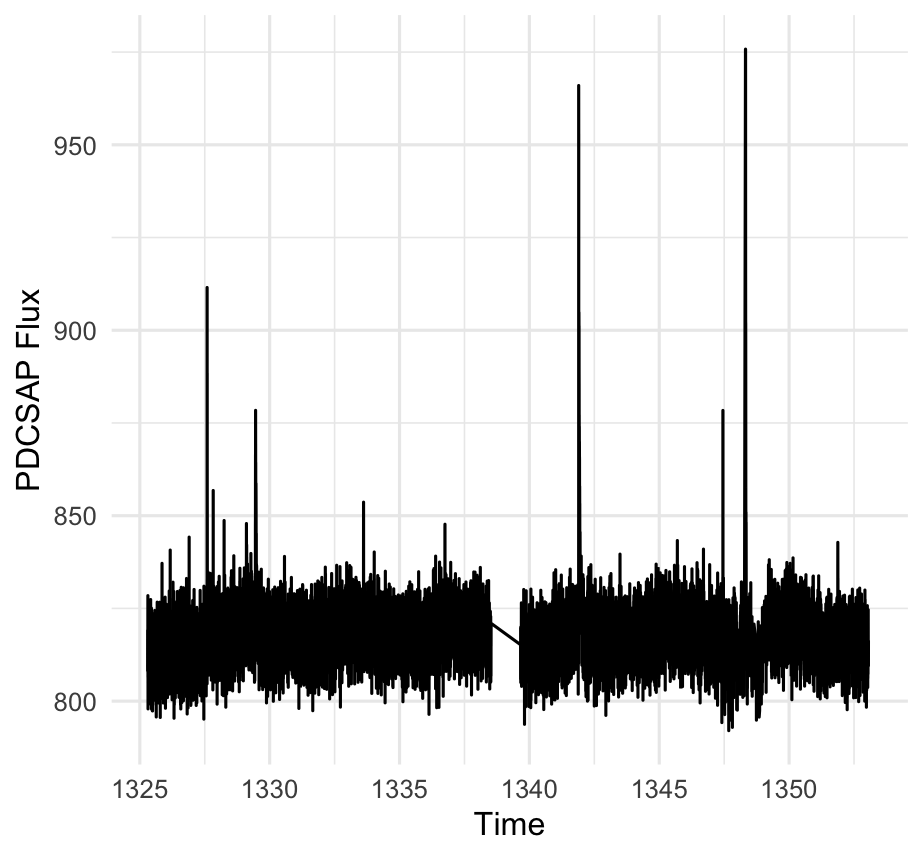
\includegraphics[width=0.5\linewidth]{Figure/ts_plot_129} }\subfloat[after\label{fig:data-2}]{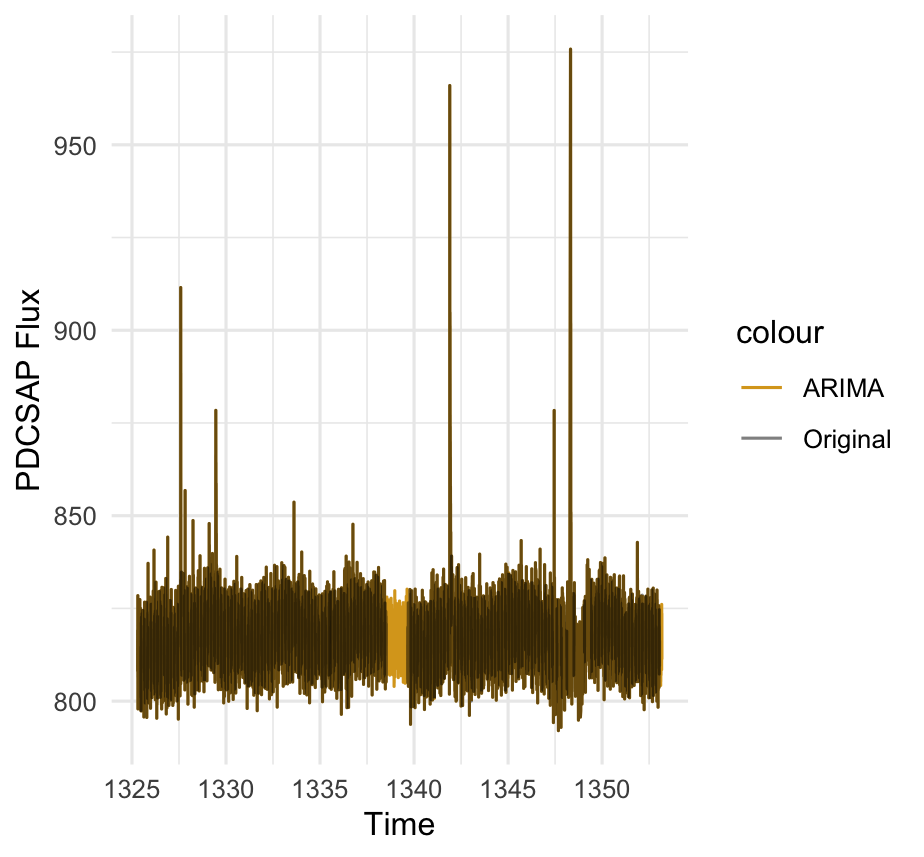
\includegraphics[width=0.5\linewidth]{Figure/ARIMA_ImputeTS_129} }

}

\caption{model results}\label{fig:data}
\end{figure}

\section{Methods}\label{methods}

\subsection{Time Series Analysis}\label{time-series-analysis}

\subsection{Machine Learning Methods}\label{machine-learning-methods}

\section{Results}\label{results}

\subsection{Time Series Model}\label{time-series-model}

\subsubsection{With Missing Value Imputation}\label{with-missing-value-imputation}

\begin{figure}[H]

{\centering \subfloat[result\label{fig:ts-1}]{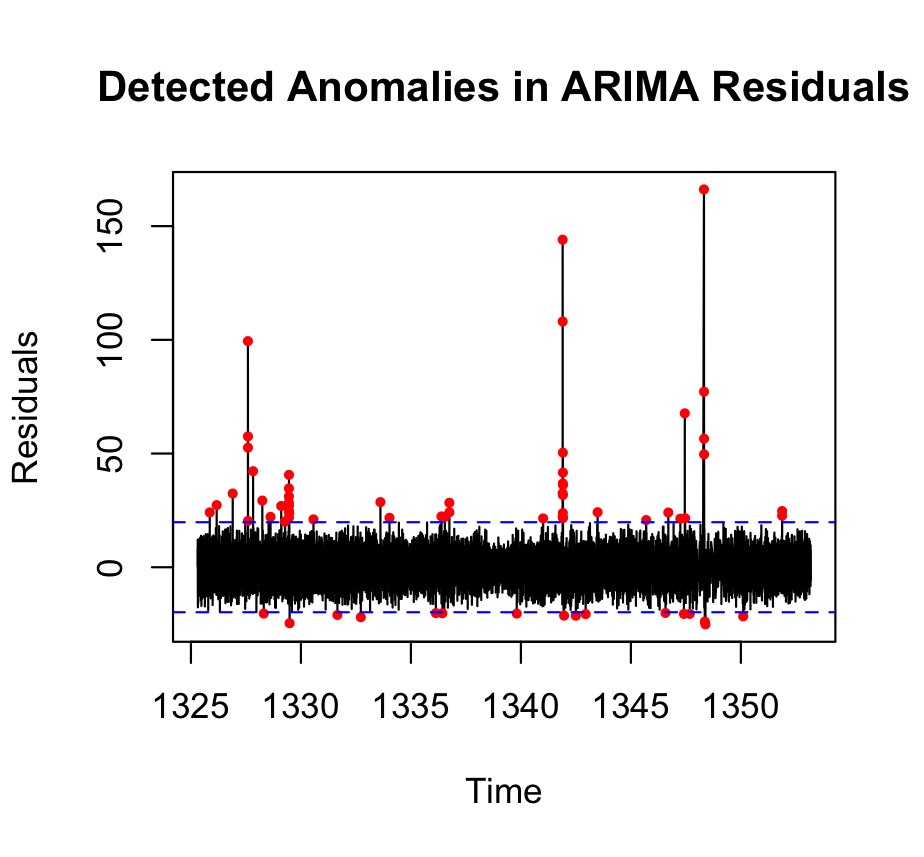
\includegraphics[width=0.5\linewidth]{Figure/arima_129} }\subfloat[residual\label{fig:ts-2}]{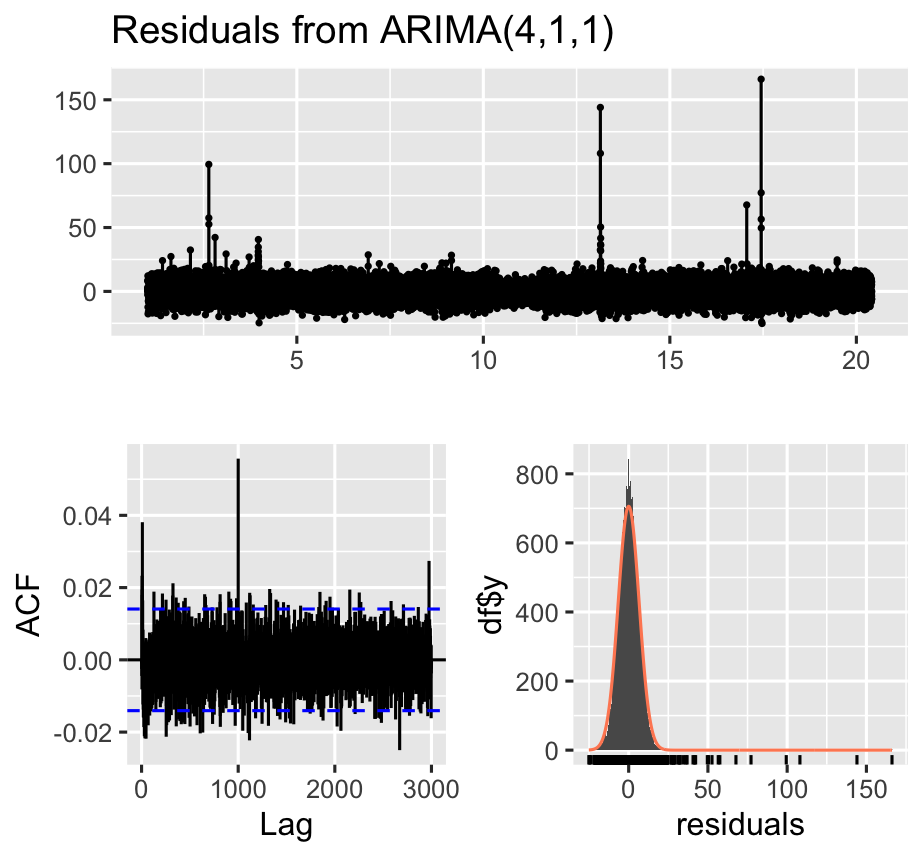
\includegraphics[width=0.5\linewidth]{Figure/res_arima_129} }

}

\caption{model results}\label{fig:ts}
\end{figure}

\subsubsection{Without Missing Value Imputation}\label{without-missing-value-imputation}

\begin{figure}[H]

{\centering \subfloat[result\label{fig:ts2-1}]{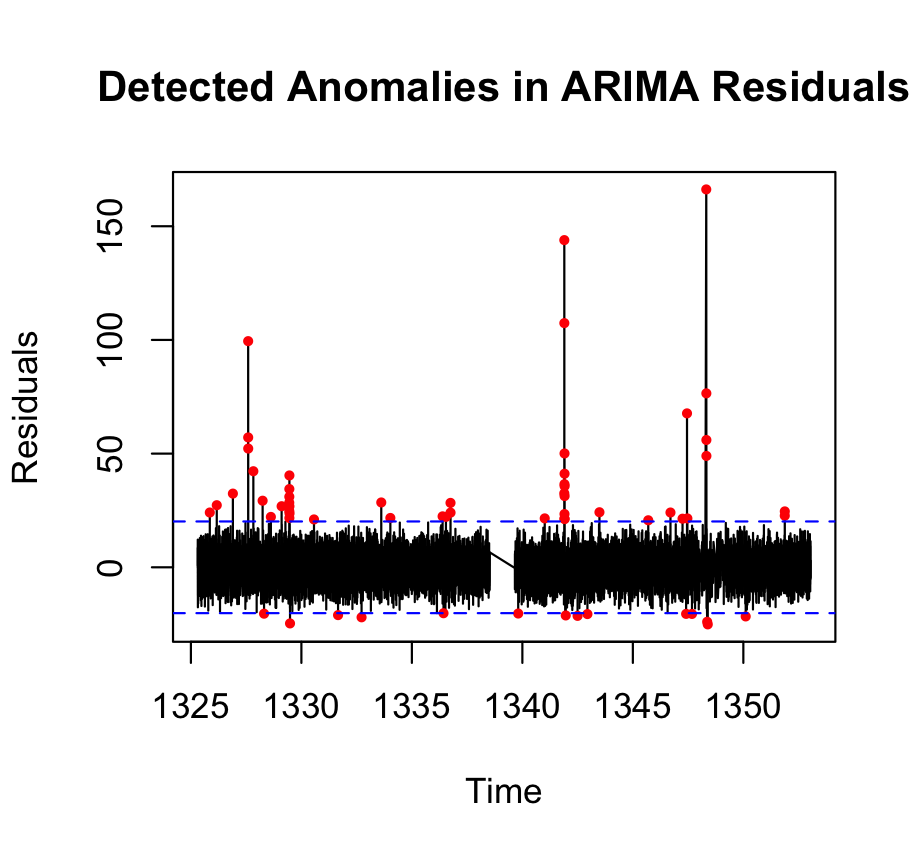
\includegraphics[width=0.5\linewidth]{Figure/arima_129_without_imputation} }\subfloat[residual\label{fig:ts2-2}]{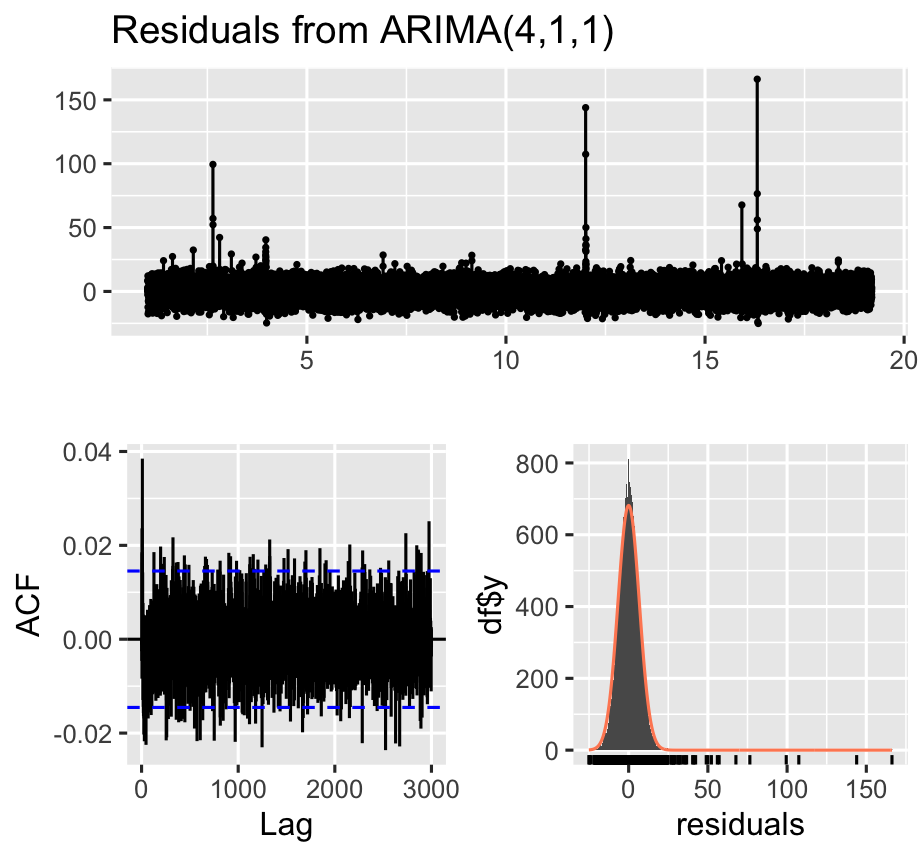
\includegraphics[width=0.5\linewidth]{Figure/res_arima_129_without_imputation} }

}

\caption{model results}\label{fig:ts2}
\end{figure}

\subsection{Machine Learning Model}\label{machine-learning-model}

\subsubsection{With Missing Value Imputation}\label{with-missing-value-imputation-1}

\begin{figure}[H]

{\centering \subfloat[if\label{fig:ml-1}]{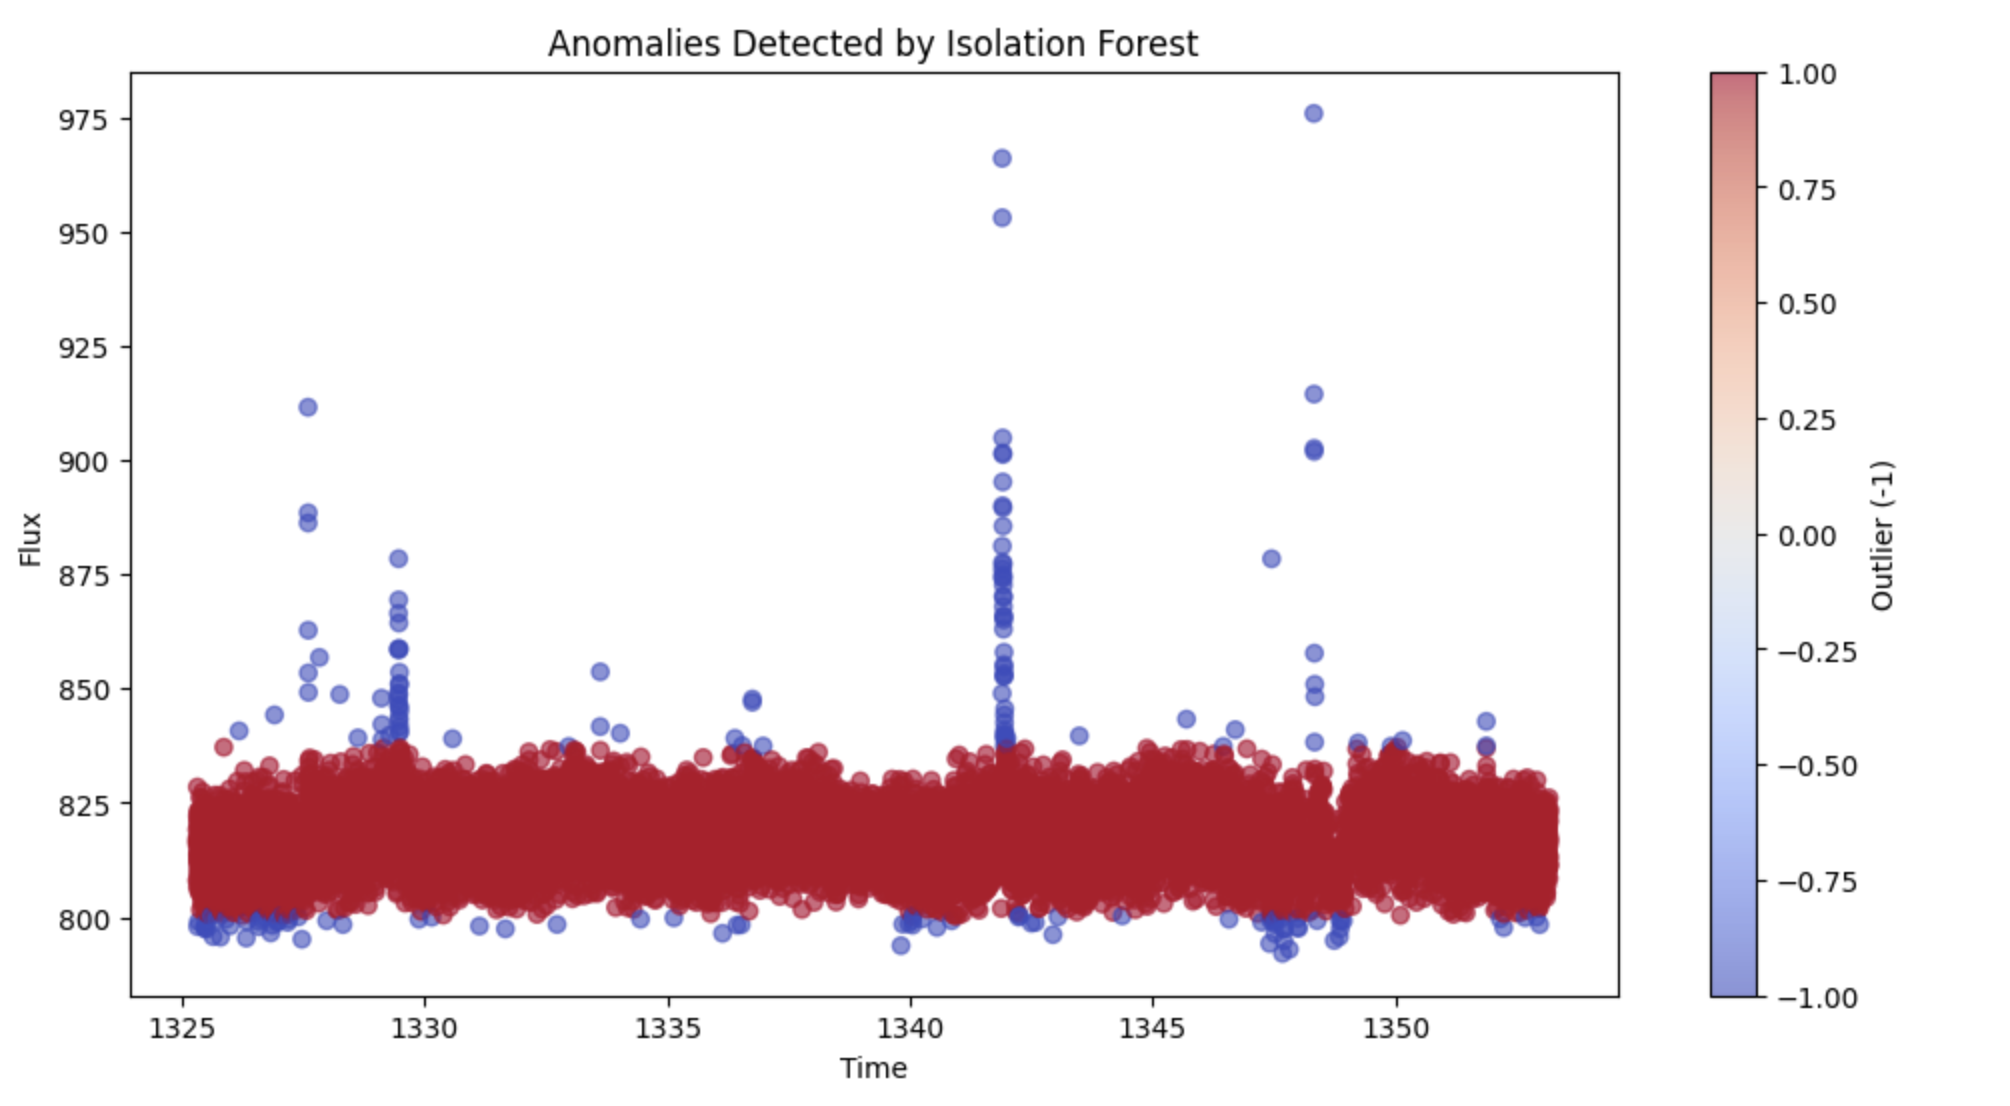
\includegraphics[width=0.5\linewidth]{Figure/IF_1_129} }\subfloat[gmm\label{fig:ml-2}]{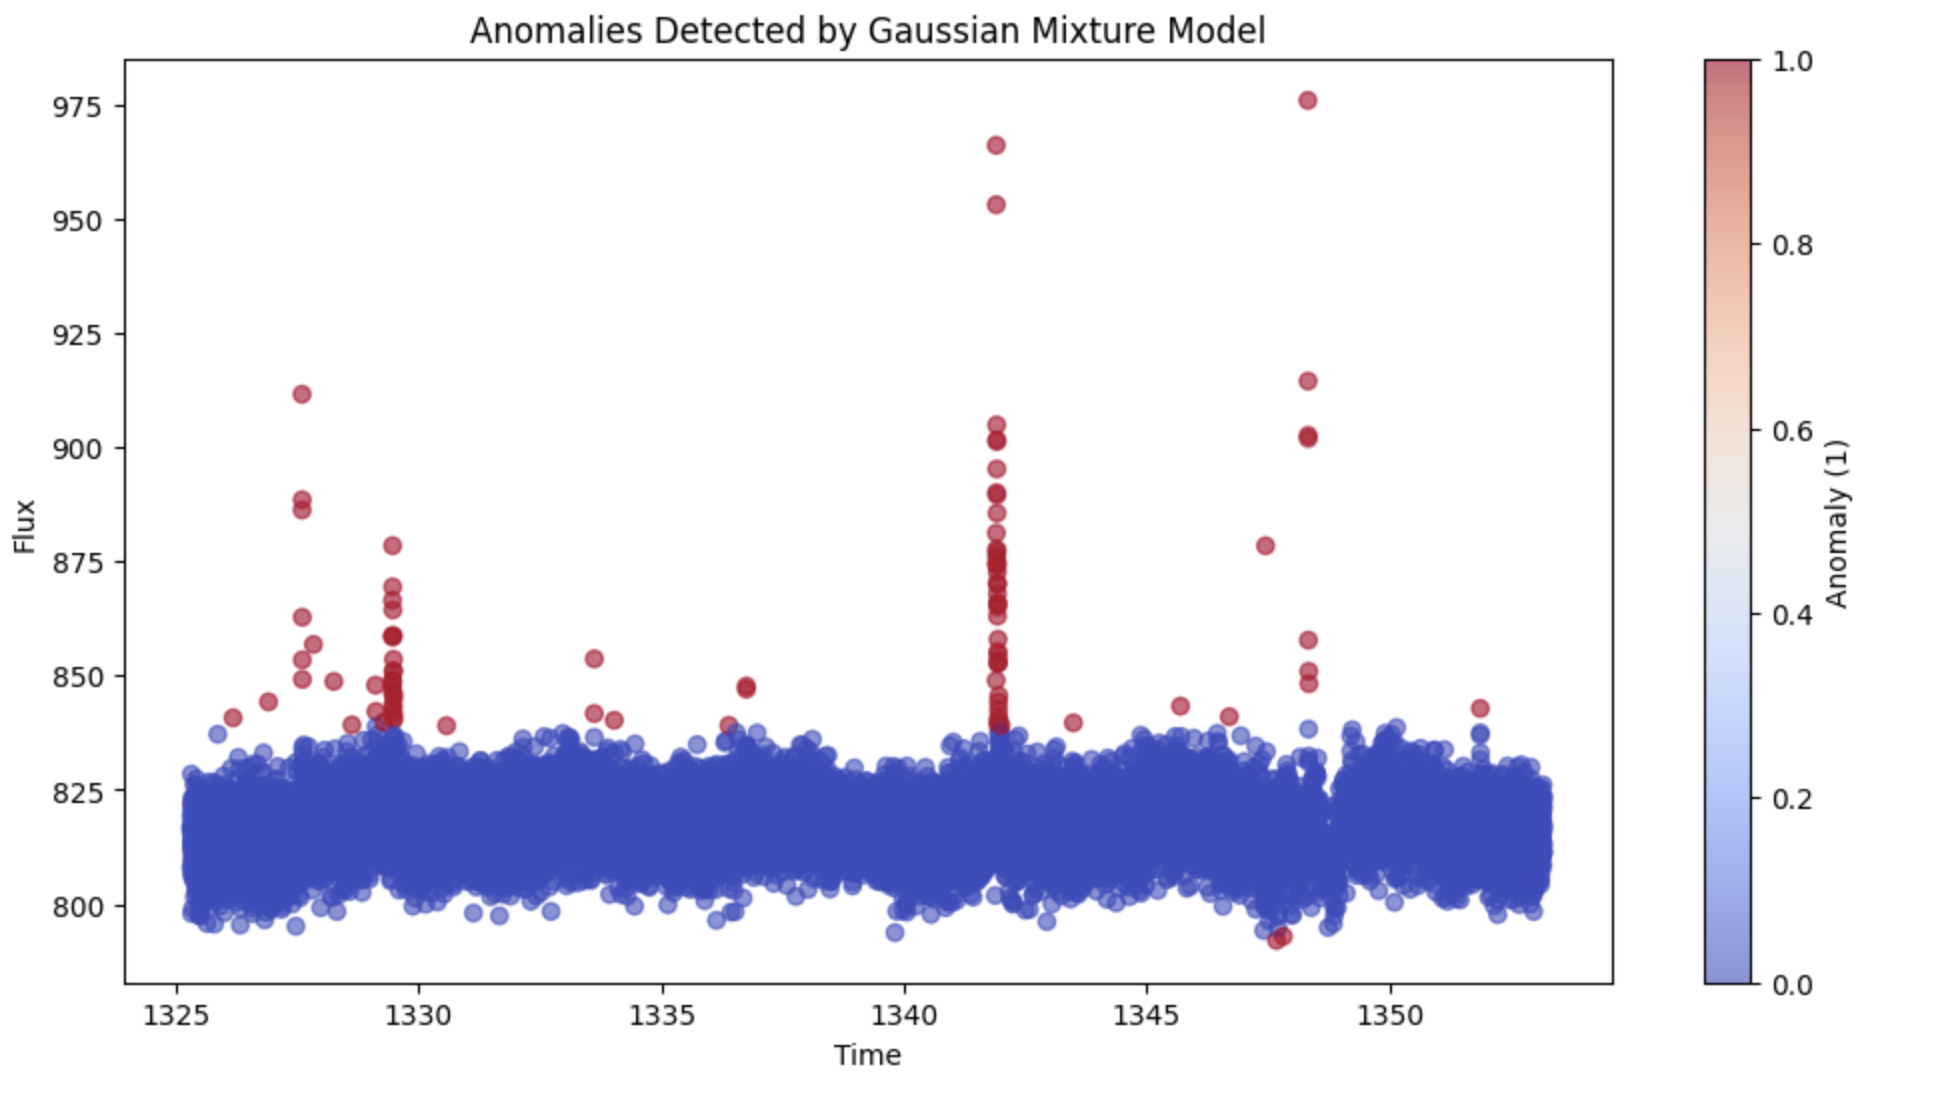
\includegraphics[width=0.5\linewidth]{Figure/GMM_1_129} }\newline\subfloat[dbscan\label{fig:ml-3}]{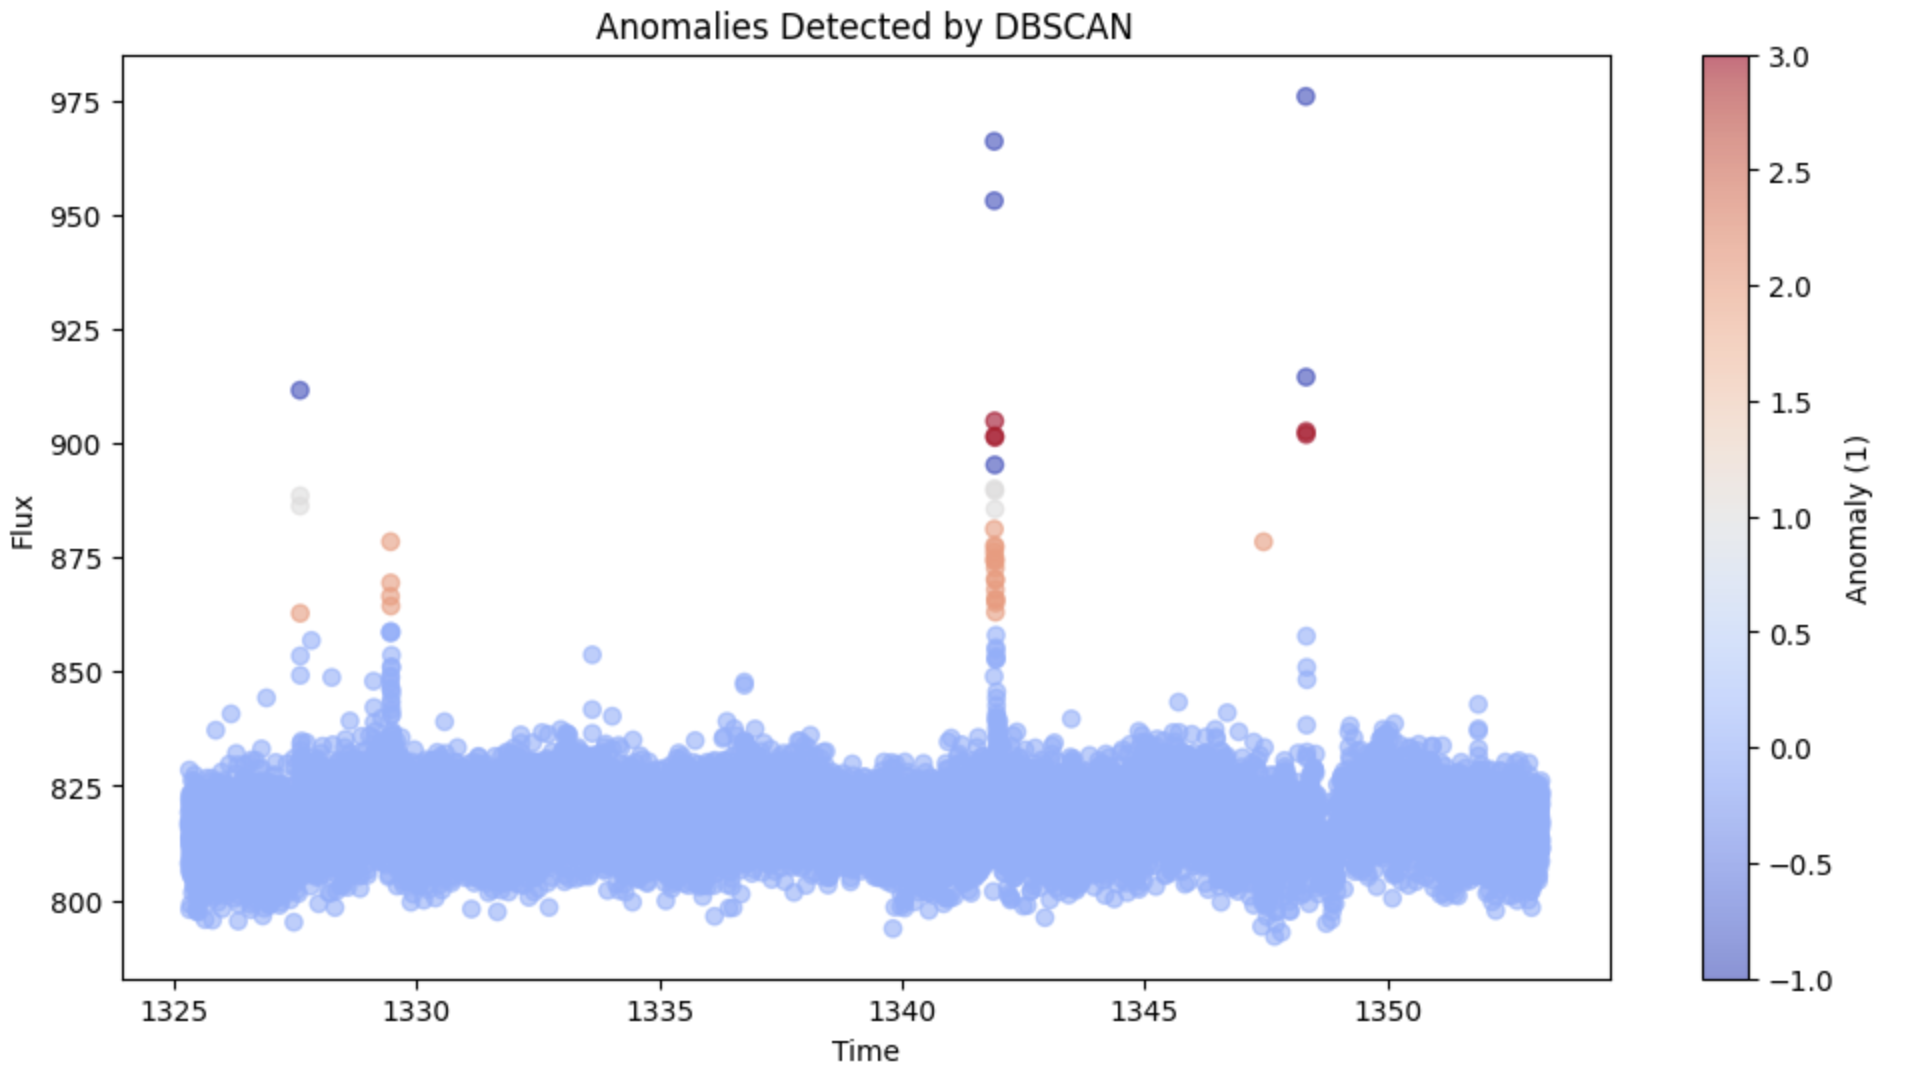
\includegraphics[width=0.5\linewidth]{Figure/DBSCAN_1_129} }

}

\caption{model results}\label{fig:ml}
\end{figure}

\subsubsection{Without Missing Value Imputation}\label{without-missing-value-imputation-1}

\begin{figure}[H]

{\centering \subfloat[if\label{fig:ml2-1}]{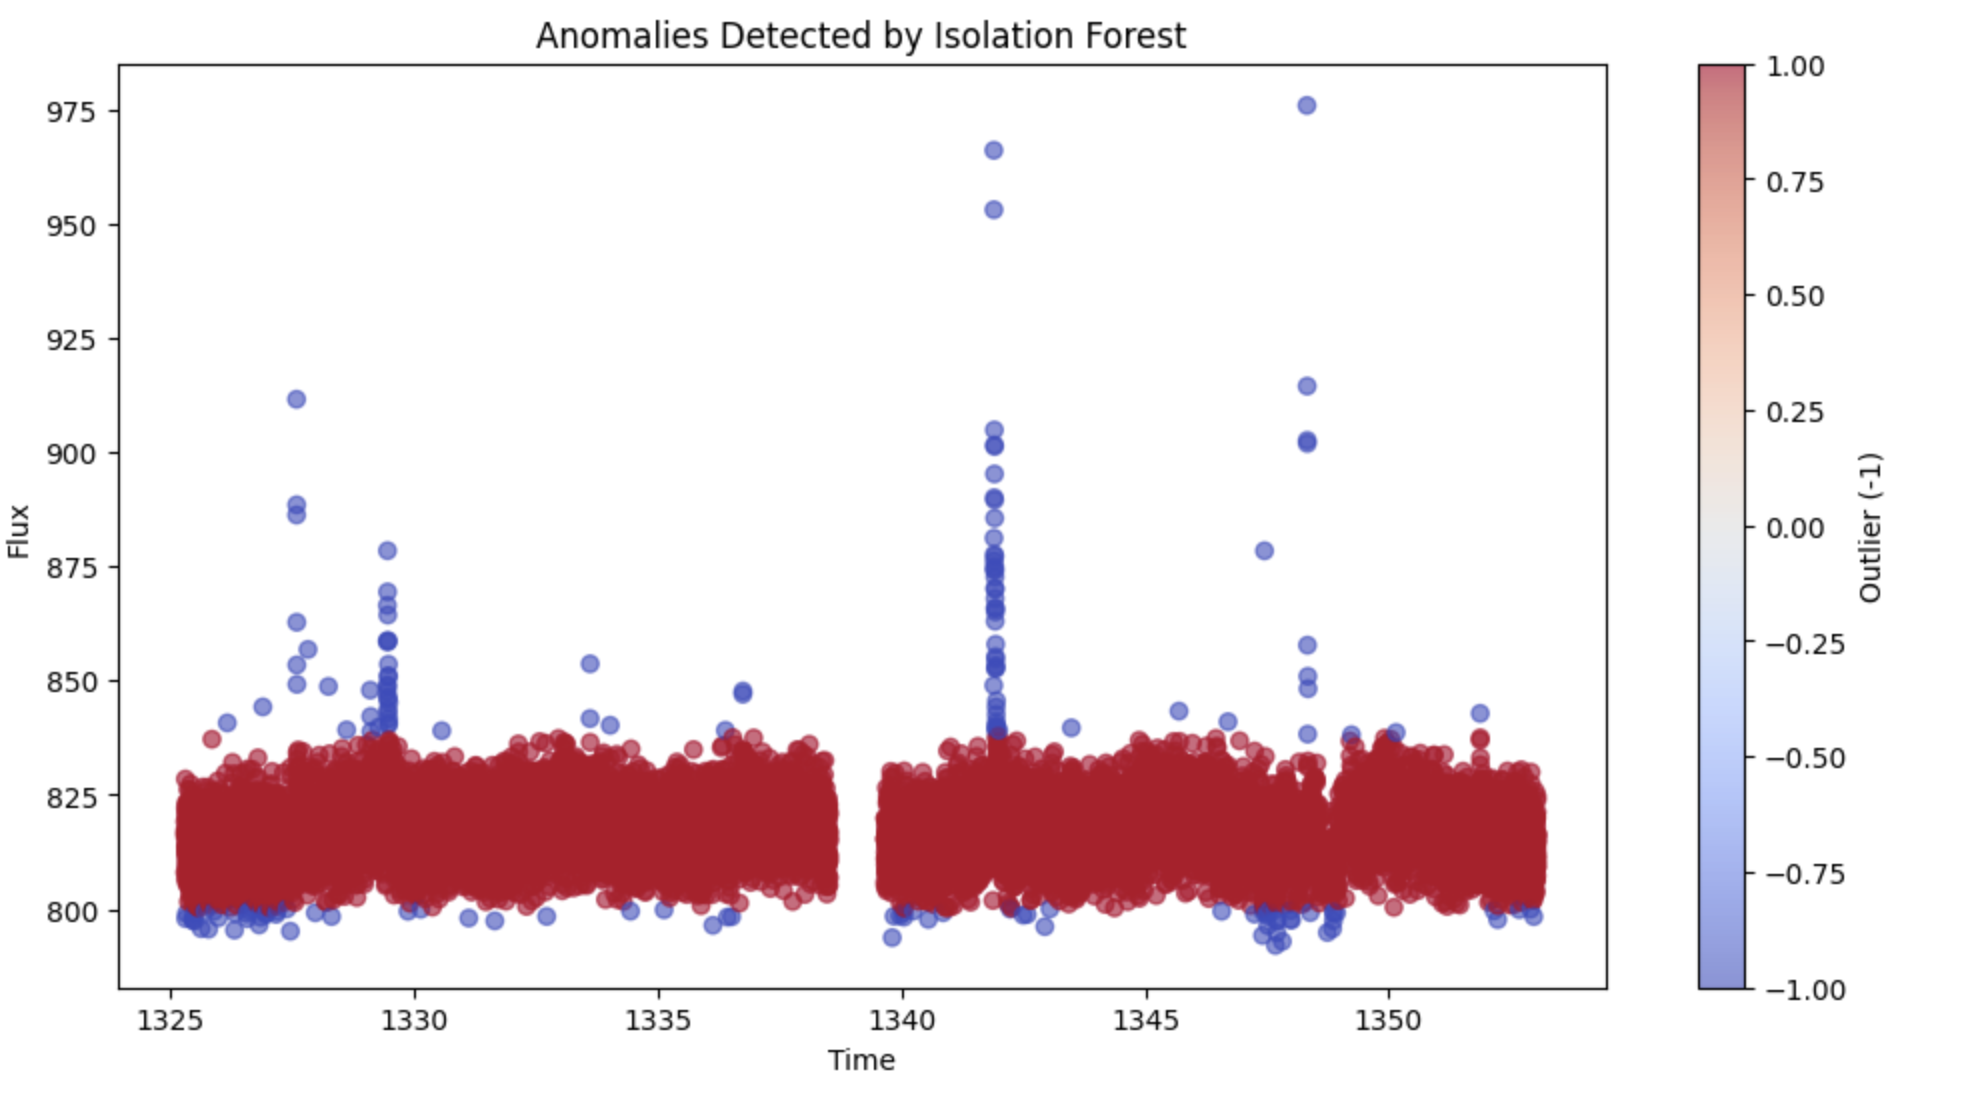
\includegraphics[width=0.5\linewidth]{Figure/IF_1_129_without_imputation} }\subfloat[gmm\label{fig:ml2-2}]{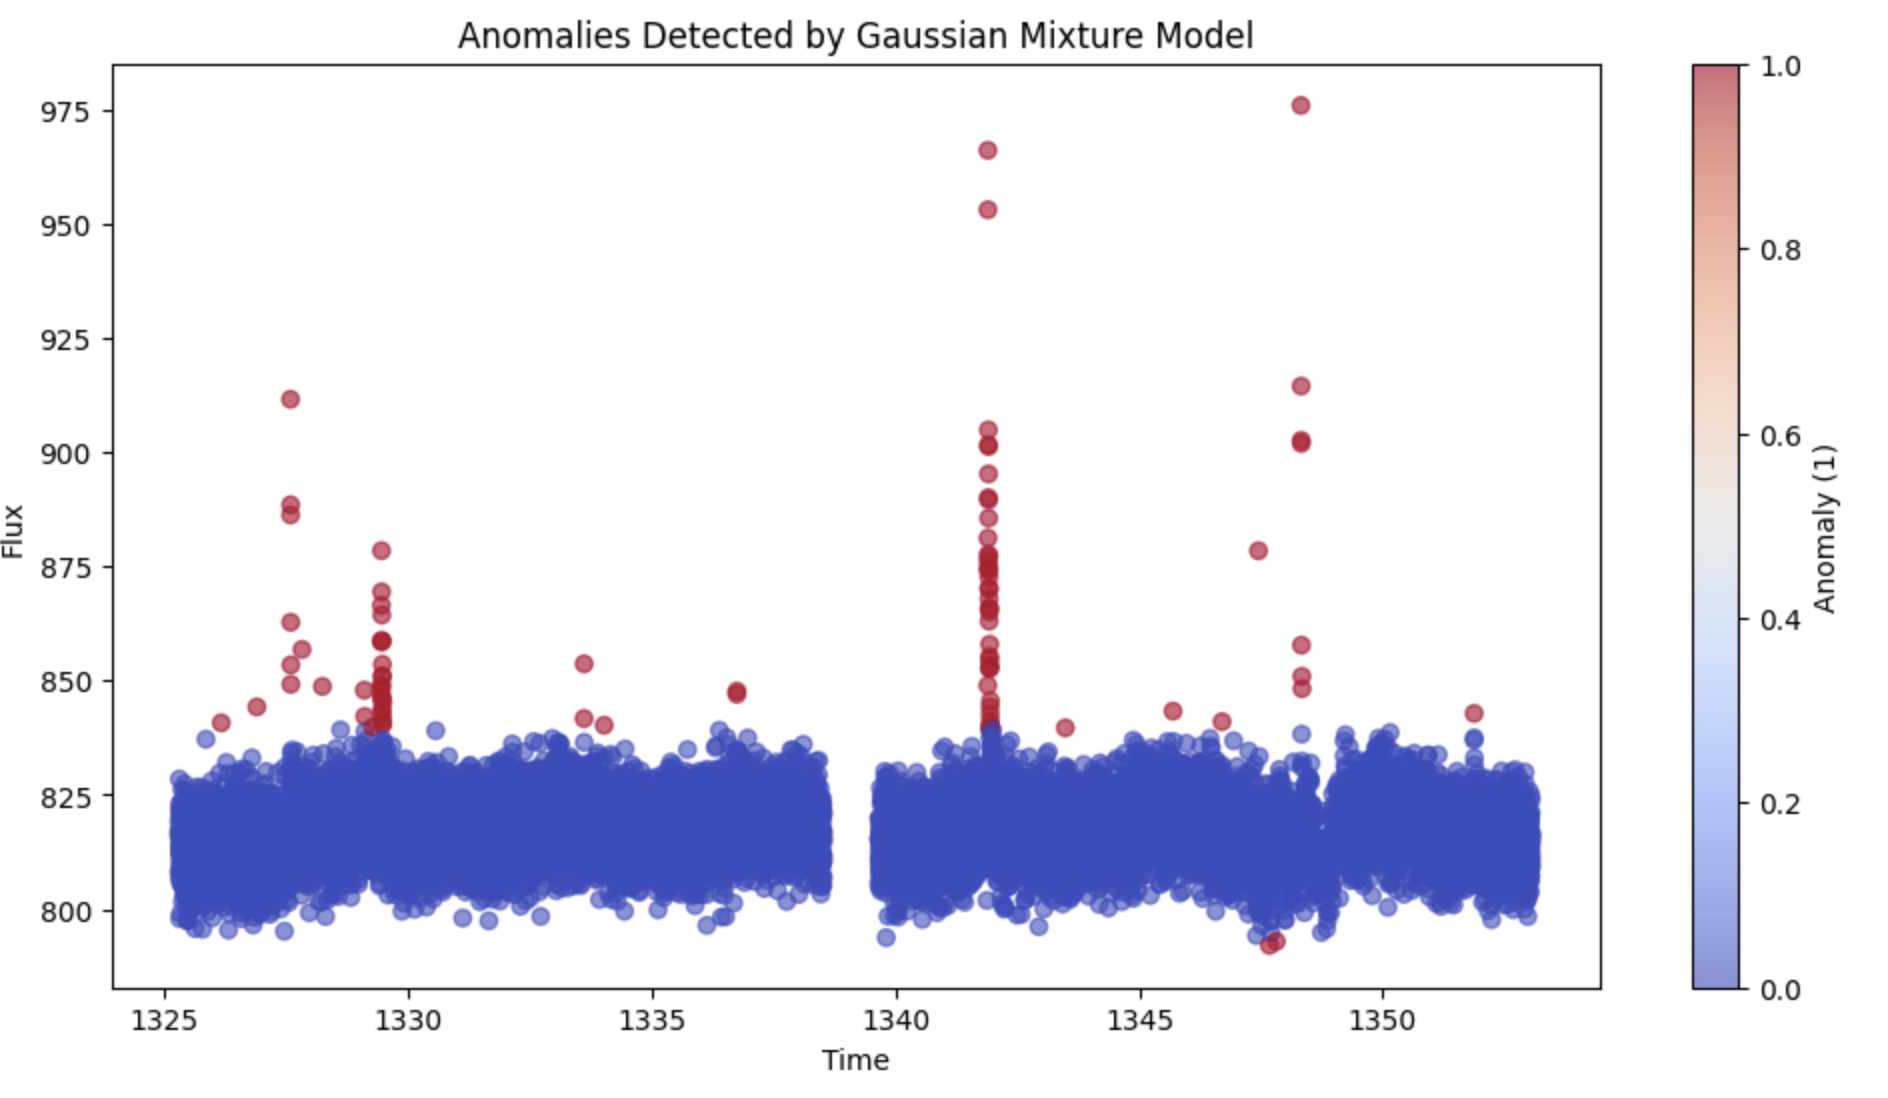
\includegraphics[width=0.5\linewidth]{Figure/GMM_1_129_without_imputation} }\newline\subfloat[dbscan\label{fig:ml2-3}]{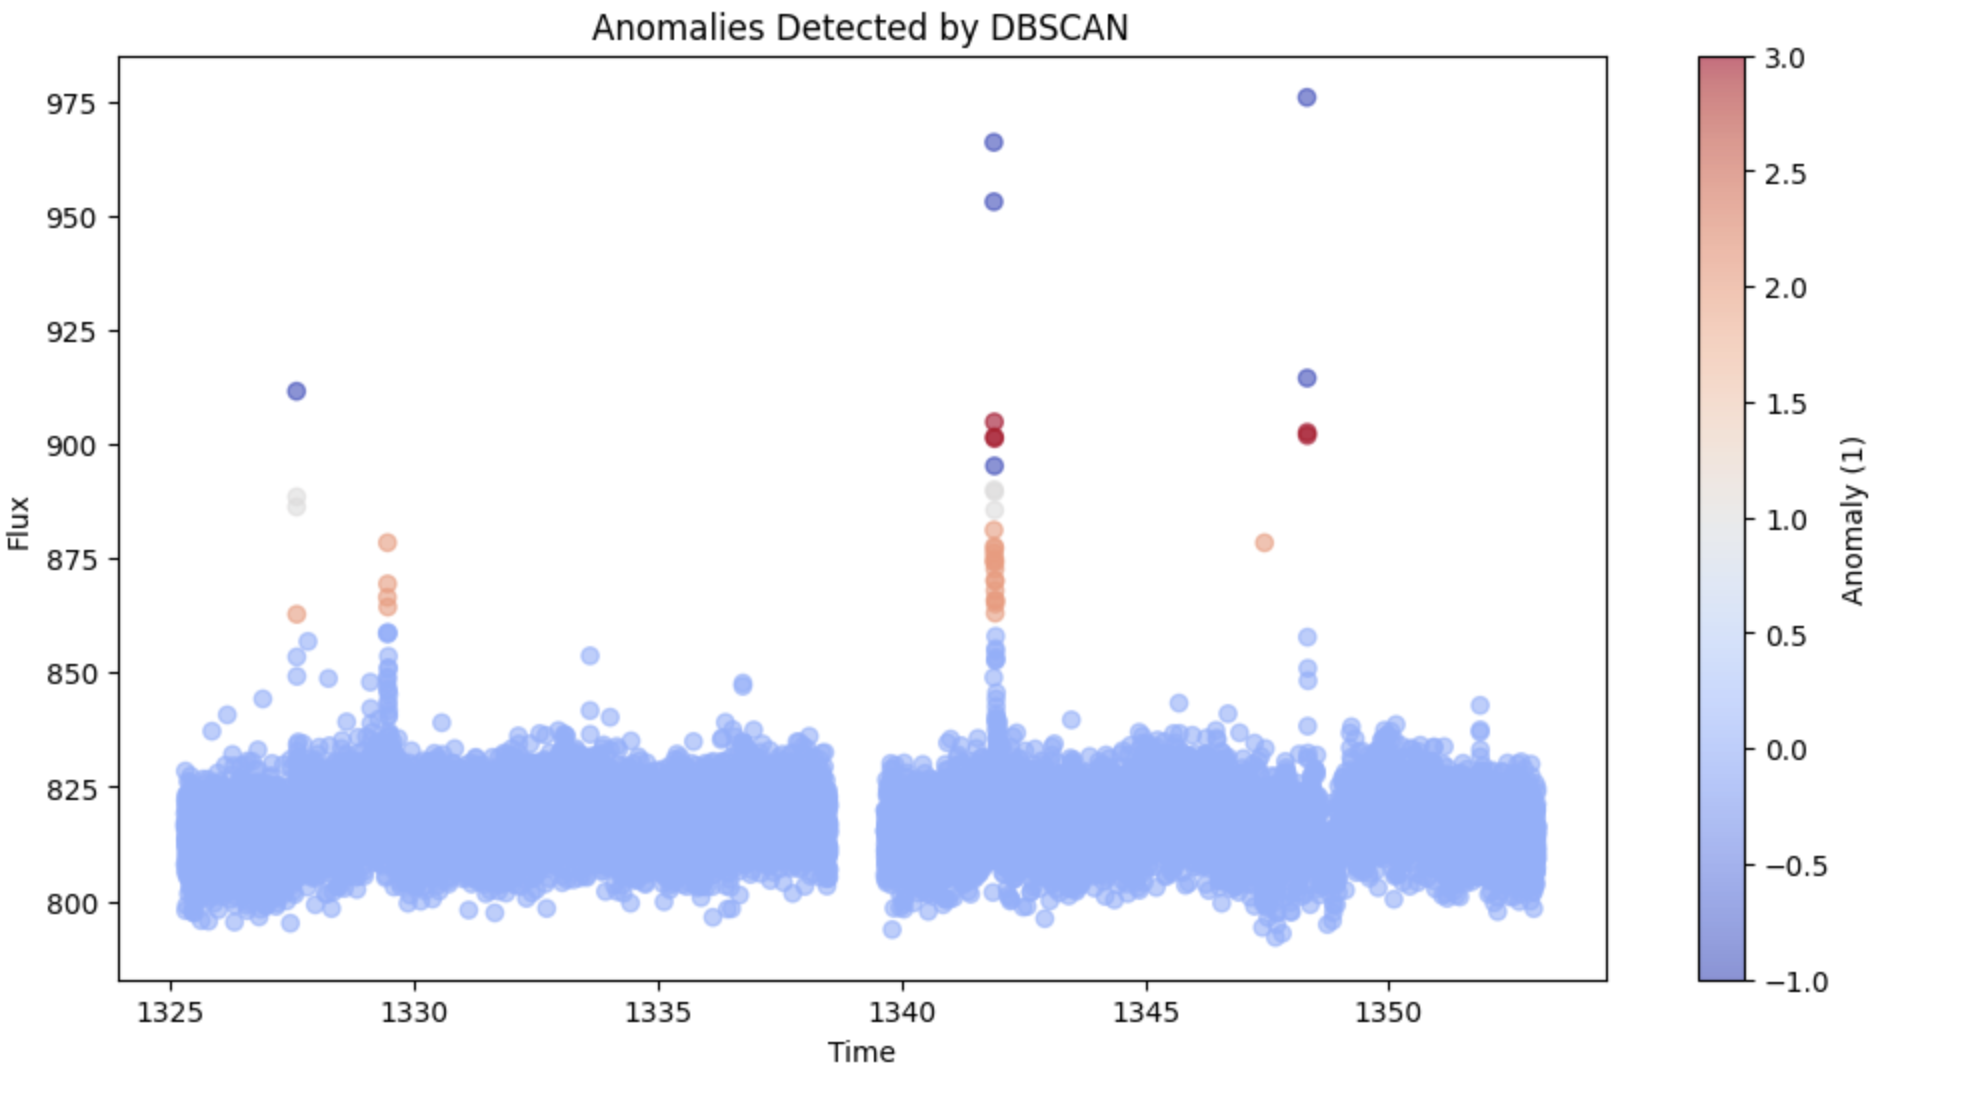
\includegraphics[width=0.5\linewidth]{Figure/DBSCAN_1_129_without_imputation} }

}

\caption{model results}\label{fig:ml2}
\end{figure}

\section{Discussion}\label{discussion}

\subsection{Current Work}\label{current-work}

decide to use no imputation data, why

\subsection{Next Steps}\label{next-steps}

Tune parameter

decide validation and metric to compare model performance

\end{document}
